\documentclass{article}
\usepackage[paper=a4paper,margin=1in]{geometry}

\usepackage{listings}
\usepackage{graphicx}

\usepackage{comment}

\usepackage{amsmath}

\usepackage{todonotes}

\newcommand{\titlelogoimage}{
\begin{figure}[h!]
	\centering
	
\includegraphics[width=1in]{images/logo.eps}
\end{figure}}

%opening
\title{SProc Instruction Set Architecture}
\author{Ian O'Rourke}
\date{\today \\ \titlelogoimage}

\lstset{basicstyle=\tiny,frame=single}

\begin{document}

\maketitle

\section{Overview}

SProc is a general-purpose Reduced Instruction Count (RISC) Instruction Set Architecture (ISA). Each program instruction is designed to take up exactly one word of memory. In this case, each word is 16-bits, with the primary data type being integers. In cases where signed arithmatic is performed, signed integers are encoded using the two's-complement format.

\subsection{Registers}

There are 16 total registers present on the SProc. These are defined generally as follows in Table \ref{table:register-setup}. Note that, as SProc is a 16-bit architecture, this means that each register is 16 bits wide.

\begin{table}[h!]
	\centering
	\begin{tabular}{c|c}
		\hline
		Register & Usage \\
		\hline
		R0 & Program Counter \\
		R1 & Global Stack Pointer \\
		R2 & Return Value \\
		R3 & Processor Status Flags \\
		R4-R15 & General Purpose Register \\
		\hline
	\end{tabular}
	\caption{Outside of the program counter and global stack pointer, the registers within the SProc are all general-purpose.}
	\label{table:register-setup}
\end{table}

The program counter indicates the next instruction to be read. At the beginning of the processor cycle, the instruction at the memory address of the program counter is read in and processed. Then, the program counter is incremented at the end of each instruction cycle. If this value is needed to be modified, it is recommended to use the absolute jump instruction, \texttt{jmp}, or the relative jump instruction, \texttt{jmpr}.

The global stack pointer maintains the global stack, as defined in Section \ref{sec:the-stack}. This provides the offset from the stack's base address right off-the-end of the current stack contents. Thus, when the stack is empty, it points to the stack base address, and when the stack is completely full it points to the memory location just above the last stack entry, or the base address plus the stack size. This value should not be edited by-hand to maintain the consistency of the program execution, but is instead modified by the stack instructions \texttt{push}, \texttt{pop}, \texttt{popr}, \texttt{call}, \texttt{ret}, \texttt{retint}, and \texttt{int}, as well as hardware interrupts.

The return value instruction is intended to store the result of a function call, made using the \texttt{call} instruction. When the processor status flags are replaced with the caller's flags after the \texttt{ret} instruction is called, the return value is the only register that remains unchanged.

The processor status flags indicate the current setup for the processor. Currently, the following flags are assigned, as noted in Table \ref{table:processor-flags}.

\begin{table}[h!]
	\centering
	\begin{tabular}{l|l}
		\hline
		Bit & Value \\
		\hline
		0 & Interrupt Enable \\
		1 & Signed Relational Operators \\
		\hline
	\end{tabular}
	\caption{Processor status flags provide a window into the current processor state}
	\label{table:processor-flags}
 \end{table}

This provides both a means to set and to read the current processor state values to ensure that the proper operating mode is configured for the currently-running program. This is maintained and replaced when \texttt{ret} and \texttt{retint} are called, so within an interrupt or function call, it is not necessary to replace the processor flags with those of the caller.

\subsection{Overall Instruction Syntax}

Since the architecture of the SProc is 16-bit, this means that each word that may be addressed is 16-bits. The general instruction format is listed  in Table \ref{table:instruction-formatting}.

\begin{table}[h!]
	\centering
	\begin{tabular}{l|cccc}
		\hline
		Location & 0xF000 & 0x0F00 & 0x00F0 & 0x000F \\
		\hline
		Usage & opcode & arg0 & arg1 & arg2 \\
		\hline
	\end{tabular}
	\caption{The SProc instruction format typically has one opcode and three possible arguments associated with a particular opcode}
	\label{table:instruction-formatting}
\end{table}

This is contrasted with the typical assembly language formatting, which is provided as

\begin{center}
	\texttt{instruction <arg2>, <arg1>, <arg0>}
\end{center}

where the number of arguments depends on the required number of arguments for the instruction.

\subsection{Resetting}

On a hard-reset, all registers will be reset to 0 and memory values will be reset to their default values. The data parameter in memory at the hard-reset vector, stored at memory location 0, will be used as the reset vector.

On soft-reset, as called by the reset the program counter will be assigned the value contained in the soft-reset vector, which is stored at memory location 1. All of the other registers are reset to their default value of 0. Processor memory will be left unchanged and processor execution is then started.

On any reset, interrupts will be allowed by default.

\subsection{The Stack}
\label{sec:the-stack}

The stack pointer provides an offset from the stack pointer starting location. By default, this is at memory location 0x400. The stack pointer may grow up to a size of 0xC00, or 3072, items. This provides a maximum stack address of 0x1000. If the stack pointer is ever popped such that its value would underflow 0 or would reach greater than the maximum allowed size, the processor will error and halt.

\subsection{Interrupts}

Interrupts provide a means to interrupt the current flow of execution and run a separate method. There are two types of interrupts - hardware interrupts, which originate by request of an external hardware device, and software interrupts, which originate from a specific instruction. When an interrupt is triggered, the flow of program execution is interrupted before the next instruction is started. The current register state is stored on the stack, and the program counter is replaced with the value in the corresponding interrupt vector. Then, the program execution continues from this new location.

At the conclusion of any interrupt, the \texttt{retint} instruction should be called. This will replace the current register state with the values provided off the stack and resume program execution from the location right after the interrupt was called.

It should be noted that, if any values were pushed onto the stack during the interrupt handler, they should be popped off the stack prior to the \texttt{retint} call to avoid corrupting the program state.

The SProc supports up to 16 software interrupts and up to 16 hardware interrupts, as shown in Table \ref{table:interrupt-vector-locations}. Software interrupt vectors are stored in memory at location \texttt{0x2} for software interrupt 0 though \texttt{0x12}, exclusive. Similarly, the 16 hardware interrupts are stored in memory at memory address \texttt{0x12} through \texttt{0x22}, exclusive.

\begin{table}[h!]
	\centering
	\begin{tabular}{c|ccccccc}
		\hline
		Type & 0 & 1 & 2 & \dots & 13 & 14 & 15 \\
		\hline
		Software & \texttt{0x2} & \texttt{0x3} & \texttt{0x4} & \dots & \texttt{0xF} & \texttt{0x10} & \texttt{0x11} \\
		Hardware & \texttt{0x12} & \texttt{0x13} & \texttt{0x14} & \dots & \texttt{0x1F} & \texttt{0x20} & \texttt{0x21} \\
		\hline
	\end{tabular}
	\caption{Interrupt vector locations for both hardware and software interrupts}
	\label{table:interrupt-vector-locations}
\end{table}

Note that, if a vector has a value of zero, that interrupt vector is considered to be disabled and that interrupt will effectively be disabled and not able to be run.

\pagebreak

\section{Instructions and Assembly Code}

All available instructions are listed in Table \ref{table:instruction-table}. Note that any invalid instruction that is not provided in the table below results in an immediate halt of the processor. Note that, in the below logic, any indication where PC is incremented indicates that the standard \texttt{PC += 1} to move to the next instruction will be replaced by the logic provided in the description field. \todo{combine left/right shift?} \todo{add load reg = base + offset?} \todo{keep bxor?} \todo{test equal}

\begin{table}[h!]
	\centering
	\begin{footnotesize}
		\begin{tabular}{cccc|c|l}
			\hline
			\multicolumn{4}{c|}{Instruction Word} & Assembly & Description \\
			opcode & arg0 & arg1 & arg2 & & \\
			\hline
			0 & 0 & 0 & 0 & \texttt{noop} & No Operation \\
			0 & 0 & 0 & 1 & \texttt{inton} & Turn Interrupts On \\
			0 & 0 & 0 & 2 & \texttt{intoff} & Turn Interrupts Off \\
			0 & 0 & 0 & 3 & \texttt{reset} & \texttt{PC = Reset Vector}, \texttt{R[0-15] = 0} \\
			0 & 0 & 0 & 4 & \texttt{pop} & \texttt{--SP} \\
			0 & 0 & 0 & 5 & \texttt{ret} & \texttt{x = R[ret]} \\
			{} & {} & {} & {} & {} & $\forall_{i \in [15 \rightarrow 0]}$ \texttt{R[i] = mem[--SP]}, \texttt{++PC} \\
			{} & {} & {} & {} & {} & \texttt{R[ret] = x} \\
			0 & 0 & 0 & 6 & \texttt{retint} & $\forall_{i \in [15 \rightarrow 0]}$ \texttt{R[i] = mem[--SP]}, \texttt{++PC} \\
			0 & 0 & 1 & R[a] & \texttt{jmp [a]} & \texttt{PC = R[a]} \\
			0 & 0 & 2 & R[a] & \texttt{jmpr [a]} & \texttt{PC += R[a]} \\
			0 & 0 & 3 & R[a] & \texttt{push [a]} & \texttt{mem[SP++] = R[a]} \\
			0 & 0 & 4 & R[a] & \texttt{popr [a]} & \texttt{R[a] = mem[--SP]} \\
			0 & 0 & 5 & R[a] & \texttt{call [a]} & $\forall_{i \in [0 \rightarrow 15]}$
			 \texttt{mem[SP++] = R[i]}, \texttt{PC = R[a]} \\
 			0 & 0 & 6 & 0xI & \texttt{int <imm>} & Trigger software interrupt number \texttt{imm} \\
 			0 & 0 & 7 & R[a] & \texttt{intr [a]} & Trigger software interrupt number in \texttt{R[a]} \\
 			0 & 0 & 8 & R[a] & \texttt{tz [a]} & If \texttt{R[a] == 0} \texttt{PC += 1}, Else \texttt{PC += 2} \\
 			0 & 0 & 9 & R[a] & \texttt{tnz [a]} & If \texttt{R[a] != 0} \texttt{PC += 1}, Else \texttt{PC += 2} \\
 			0 & 0 & 10 & R[a] & \texttt{bool [a]} & If \texttt{R[a] != 0} \texttt{R[a] = 1}, Else \texttt{R[a] = 0} \\
 			0 & 0 & 11 & R[a] & \texttt{not [a]} & If \texttt{R[a] != 0} \texttt{R[a] = 0}, Else \texttt{R[a] = 1} \\
			0 & 1 & 0xI0 & 0x0I & \texttt{jmpri <imm>} & \texttt{PC += Im} \\
			0 & 2 & R[src] & R[dst] & \texttt{ld [dst], [src]} & \texttt{R[dst] = mem[R[src]]} \\
			0 & 3 & R[src] & R[dst] & \texttt{sav [dst], [src]} & \texttt{mem[R[dst]] = R[src]} \\
			0 & 4 & R[src] & R[dst] & \texttt{ldr [dst], [src]} & \texttt{R[dst] = mem[PC + R[src]]} \\
			0 & 5 & R[src] & R[dst] & \texttt{savr [dst], [src]} & \texttt{mem[PC + R[dst]] = R[src]} \\
			0 & 6 & R[b] & R[a] & \texttt{copy [a], [b]} & \texttt{R[a] = R[b]} \\
			0 & 7 & R[b] & R[a] & \texttt{tg [a], [b]} & If \texttt{R[a] > R[b]} \texttt{PC += 1}, Else \texttt{PC += 2} \\
			0 & 8 & R[b] & R[a] & \texttt{tge [a], [b]} & If \texttt{R[a] >= R[b]} \texttt{PC += 1}, Else \texttt{PC += 2} \\
			0 & 9 & R[b] & R[a] & \texttt{tl [a], [b]} & If \texttt{R[a] < R[b]} \texttt{PC += 1}, Else \texttt{PC += 2} \\
			0 & 10 & R[b] & R[a] & \texttt{tle [a], [b]} & If \texttt{R[a] >= R[b]} \texttt{PC += 1}, Else \texttt{PC += 2}\\
			0 & 11 & R[b] & R[a] & \texttt{bnot [a], [b]} & \texttt{R[a] = ~R[b]} \\
			0 & 12 & 0x0I & R[a] & \texttt{arg [a], <imm>} & \texttt{R[a] = SP - 16 - 1 - Im} \\
			1 & 0xI0 & 0x0I & R[dst] & \texttt{ldi [dst], <imm>} & \texttt{R[dst] = Im} \\
			2 & 0xI0 & 0x0I & R[dst] & \texttt{ldui [dst], <imm-unsigned>} & \texttt{R[dst] = Im} \\
			3 & 0xI0 & 0x0I & R[dst] & \texttt{ldir [dst], <imm>} & \texttt{R[dst] = mem[PC + Im]} \\
			4 & R[b] & R[a] & R[dst] & \texttt{add [dst], [a], [b]} & \texttt{R[dst] = R[a] + R[b]} \\
			5 & R[b] & R[a] & R[dst] & \texttt{sub [dst], [a], [b]} & \texttt{R[dst] = R[a] - R[b]} \\
			6 & R[b] & R[a] & R[dst] & \texttt{mul [dst], [a], [b]} & \texttt{R[dst] = R[a] * R[b]} \\
			7 & R[b] & R[a] & R[dst] & \texttt{div [dst], [a], [b]} & \texttt{R[dst] = R[a] / R[b]} \\
			8 & R[b] & R[a] & R[dst] & \texttt{mod [dst], [a], [b]} & \texttt{R[dst] = R[a] \% R[b]} \\
			9 & R[b] & R[a] & R[dst] & \texttt{band [dst], [a], [b]} & \texttt{R[dst] = R[a] \& R[b]} \\
			10 & R[b] & R[a] & R[dst] & \texttt{bor [dst], [a], [b]} & \texttt{R[dst] = R[a] | R[b]} \\
			11 & R[b] & R[a] & R[dst] & \texttt{bxor [dst], [a], [b]} & \texttt{R[dst] = R[a] $\wedge$ R[b]} \\
			12 & R[b] & R[a] & R[dst] & \texttt{bsftl [dst], [a], [b]} & \texttt{R[dst] = R[a] << R[b]} \\
			13 & R[b] & R[a] & R[dst] & \texttt{bsftr [dst], [a], [b]} & \texttt{R[dst] = R[a] >> R[b]} \\
			\hline
		\end{tabular}
	\end{footnotesize}
	\caption{Available instruction list for the SProc provides a variety of commands.}
	\label{table:instruction-table}
\end{table}

\pagebreak

The assembler also has several commands available, detailed in Table \ref{table:assembler-commands}. Note that, for the \texttt{.loadtext} command, the text will be loaded in via the character map provided in Section \ref{sec:character-map}.

\begin{table}[h!]
	\centering
	\begin{tabular}{l|l}
		\hline
		Command & Description \\
		\hline
		\texttt{:[label]} & Defines a new label associated with the current memory location \\
		\texttt{.oper [offset]} & Changes the current assembly offset to the value provided \\
		\texttt{.load [num]} & Loads the data value as either an unsigned word (if in hex or positive)\\
		& or as a signed word (if negative) in the current memory location \\
		\texttt{.loadloc [label]} & Loads the data index associated with the provided label into \\
		& the current memory location \\
		\texttt{.loadtext "[TEXT]"} & Loads the text into memory, starting at the current memory location, \\
		& placing each character into the next subsequent memory location, with \\
		& a null-terminator as copied into memory after the text value \\
		\hline
	\end{tabular}
	\caption{Available assembler commands}
	\label{table:assembler-commands}
\end{table}

Reference names are available to link to the special register values, as listed in Table \ref{table:assembler-register-references}.

\begin{table}[h!]
	\centering
	\begin{tabular}{l|cl}
		\hline
		Reference Name & Register & Description \\
		\hline
		\texttt{\$pc} & 0 & Program Counter \\
		\texttt{\$sp} & 1 & Stack Pointer \\
		\texttt{\$ret} & 2 & Return Value \\
		\texttt{\$stat} & 3 & Status Flags \\
		\hline
	\end{tabular}
	\caption{Assembler provides shortcuts for commonly-referenced register indices}
	\label{table:assembler-register-references}
\end{table}

\pagebreak

\section{Character Mapping}
\label{sec:character-map}

SProc computers, by default, utilize the following character map. This is similar to the American Standard Code for Information Interchange (ASCII) format. The SProc character map is defined in Table \ref{table:sproc-character-map}. Any undefined entries in the character map are considered invalid characters.

\newcommand{\charmap}[1]{\texttt{#1}}

\newcommand{\charslash}{\texttt{\char`\\}}

\newcommand{\charmapescape}[1]{\charmap{\texttt{\charslash#1}}}

\begin{table}[h!]
	\centering
	\begin{tabular}{cc|cc|cc|cc}
		\hline
		Hex & Char & Hex & Char & Hex & Char & Hex & Char \\
		\hline
		00 & \charmapescape{0} NULL & 20 & Space & 40 & \charmap{@} & 60 & \charmap{`} \\
		01 & {} & 21 & \charmap{!} & 41 & \charmap{A} & 61 & \charmap{a} \\
		02 & {} & 22 & \charmap{"} & 42 & \charmap{B} & 62 & \charmap{b} \\
		03 & {} & 23 & \charmap{\#} & 43 & \charmap{C} & 63 & \charmap{c} \\
		04 & {} & 24 & \charmap{\$} & 44 & \charmap{D} & 64 & \charmap{d} \\
		05 & {} & 25 & \charmap{\%} & 45 & \charmap{E} & 65 & \charmap{e} \\
		06 & {} & 26 & \charmap{\&} & 46 & \charmap{F} & 66 & \charmap{f} \\
		07 & {} & 27 & \charmap{\textquotesingle} & 47 & \charmap{G} & 67 & \charmap{g} \\
		08 & {} & 28 & \charmap{(} & 48 & \charmap{H} & 68 & \charmap{h} \\
		09 & {} & 29 & \charmap{)} & 49 & \charmap{I} & 69 & \charmap{i} \\
		0A & \charmapescape{n} New Line & 2A & \charmap{*} & 4A & \charmap{J} & 6A & \charmap{j} \\
		0B & {} & 2B & \charmap{+} & 4B & \charmap{K} & 6B & \charmap{k} \\
		0C & {} & 2C & \charmap{,} & 4C & \charmap{L} & 6C & \charmap{l} \\
		0D & {} & 2D & \charmap{-} & 4D & \charmap{M} & 6D & \charmap{m} \\
		0E & {} & 2E & \charmap{.} & 4E & \charmap{N} & 6E & \charmap{n} \\
		0F & {} & 2F & \charmap{/} & 4F & \charmap{O} & 6F & \charmap{o} \\
		10 & {} & 30 & \charmap{0} & 50 & \charmap{P} & 70 & \charmap{p} \\
		11 & {} & 31 & \charmap{1} & 51 & \charmap{Q} & 71 & \charmap{q} \\
		12 & {} & 32 & \charmap{2} & 52 & \charmap{R} & 72 & \charmap{r} \\
		13 & {} & 33 & \charmap{3} & 53 & \charmap{S} & 73 & \charmap{s} \\
		14 & {} & 34 & \charmap{4} & 54 & \charmap{T} & 74 & \charmap{t} \\
		15 & {} & 35 & \charmap{5} & 55 & \charmap{U} & 75 & \charmap{u} \\
		16 & {} & 36 & \charmap{6} & 56 & \charmap{V} & 76 & \charmap{v} \\
		17 & {} & 37 & \charmap{7} & 57 & \charmap{W} & 77 & \charmap{w} \\
		18 & {} & 38 & \charmap{8} & 58 & \charmap{X} & 78 & \charmap{x} \\
		19 & {} & 39 & \charmap{9} & 59 & \charmap{Y} & 79 & \charmap{y} \\
		1A & {} & 3A & \charmap{:} & 5A & \charmap{Z} & 7A & \charmap{z} \\
		1B & {} & 3B & \charmap{;} & 5B & \charmap{[} & 7B & \charmap{\{} \\
		1C & {} & 3C & \charmap{<} & 5C & \charmap{\charslash} & 7C & \charmap{|} \\
		1D & {} & 3D & \charmap{=} & 5D & \charmap{]} & 7D & \charmap{\}} \\
		1E & {} & 3E & \charmap{>} & 5E & \charmap{\textasciicircum} & 7E & \charmap{\textasciitilde} \\
		1F & {} & 3F & \charmap{?} & 5F & \charmap{\textunderscore} & 7F & {} \\
		\hline
	\end{tabular}
	\caption{SProc character mapping}
	\label{table:sproc-character-map}
\end{table}

\pagebreak

\section{Devices}
\label{sec:devices}

Devices are memory-mapped in the SolariumProcessor. This means that reading or writing to special regions in memory facilitate the communication with these external devices. In a typical Solarium computer, the device region consists of up to 64 devices, starting at memory address \texttt{0xA000}, with each device allocating up to 32 words of memory. Not all devices will make use all the available memory slots for a given device. In these cases, a memory exception will be provided if any of these invalid addresses are read from or written to. \todo{add device ID}

\subsection{Serial Input and Output}

The serial input and output device is one of the simplest devices. It essentially consists of a device two queues, one for input, and another for output. Each of these queues has an internal buffer size of 256 words. If any words are attempted to be added to the queue once either queue is full, no additional data is read and that data is lost.

The current memory mapping structure for the serial input and output device is provided in Table \ref{table:dev-serial-io}.

\begin{table}[h!]
	\centering
	\begin{tabular}{l|ll}
		\hline
		Offset & Read/Write & Usage \\
		\hline
		\texttt{0} & Read & Provides the current input queue size \\
		\texttt{1} & Read & Pops and provides a word off the front of the input queue \\
		& & If no data is available, will return \texttt{0} by default \\
		\texttt{2} & Read & Provides the current output queue size \\
		\texttt{3} & Write & Pushes a word onto the output queue \\
		\texttt{4} & Write & Clears the input queue if the value written is nonzero \\
		\texttt{5} & Write & Clears the output queue if the value written is nonzero \\
		\hline
	\end{tabular}
	\caption{Serial Input and Output device provides a simple data structure to read and write data streams}
	\label{table:dev-serial-io}
\end{table}

\pagebreak

\section{Examples}

The following list some simple example programs that can be run on the SProc.

\subsection{Counter}

The program listed in Listing \ref{listing:example-counter} provides a basic counter. A target value is placed in register four, and the value in register three is incremented from 0 to the target value in register four by adding one to the register each loop. Once the target value has been reached and register three is equal to register four, the program halts by entering an infinite loop.

\lstinputlisting[caption={Limited counter program}, label={listing:example-counter}]{../examples/counter.smc}

\subsection{Infinite Counter}

Listing \ref{listing:example-infinite-counter} makes use of some additional functionality, including the use of the register reference names, to test register reset functionality. It also modifies the program counter outside of the standard jump command.

\lstinputlisting[caption={Infinite counter program with register reference names}, label={listing:example-infinite-counter}]{../examples/infinite_counter.smc}

\subsection{Hello World}

Listing  \ref{listing:hello-world} provides a program that will infinitely write "hello, world" to the serial device, expected to be memory-mapped into the SProc at \texttt{0xA000}. This makes use of the \texttt{.loadtext} command, which loads the text, and an additional null-terminator at the end, directly into memory. It also makes use of a print-string function call to handle printing string values to the serial output devices.

\lstinputlisting[caption={Infinite "hello, world!" program}, label={listing:hello-world}]{../examples/hello_world.smc}

\pagebreak

\subsection{Serial Echo}

Listing \ref{listing:serial-echo} provides a serial echo program, which echos any text provided by the default serial input device back out via the serial echo device. This serial device is expected to be provided at the starting location \texttt{0xA000}.

\lstinputlisting[caption={Serial echo program reads in text characters and immediately outputs via the output device}, label={listing:serial-echo}]{../examples/serial_echo.smc}

\pagebreak

\section{Solarium Processor Advanced Computing Environment}

The Solarium Processor Advanced Computing Environment, or spACE, is a higher-level language than the raw assembly that provides some nicer tools to program applications in, at the cost of being less space and time efficient than programming in assembly directly. It does offer a slightly safer method of computing, however, as it provides a more traditional function call structure, variables, and scopes that help abstract away some of the hardware and provide some simple limits on what the user is allowed to do.

The language specification is as follows.

\begin{tabular}{rl}
	Program & $\rightarrow$ \textlangle BaseStatement\textrangle \\
	BaseStatement & $\rightarrow$ \\
	& \textlangle BaseStatement\textrangle \textlangle BaseStatement\textlangle \\
	& func \texttt{FunctionName}(\texttt{Variable}[, \texttt{Variable}\dots]) \{ \textlangle Statement\textrangle \} \\
	& static VarType \texttt{Variable} = \textlangle Literal\textrangle \\
	Statement & $\rightarrow$ \\
	& int \texttt{Variable}; \\
	& uint \texttt{Variable}; \\
	& \texttt{Variable} = \textlangle Expression\textrangle; \\
	& return; \\
	& return \textlangle Expression\textrangle; \\
	& \{ \textlangle Statement\textrangle \} \\
	& if (\textlangle Expression\textrangle) \textlangle Statement\textrangle \\
	& if (\textlangle Expression\textrangle) \textlangle Statement\textrangle else \textlangle Statement\textrangle \\
	& while (\textlangle Expression\textrangle) \textlangle Statement\textrangle \\
	& \textlangle Statement\textrangle \textlangle Statement\textrangle \\
	Expression & $\rightarrow$ \\
	& \texttt{Variable} \\
	& \textlangle Literal\textrangle \\
	& \textlangle Expression\textrangle \textlangle BinaryOp\textrangle \textlangle Expression\textrangle \\
	& \textlangle UnaryOp\textrangle \textlangle Expression\textrangle \\
	& (\textlangle Expression\textrangle) \\
	& \texttt{FunctionName}([\textlangle Expression\textrangle[, \textlangle Expression\textrangle,\dots]]) \\
	BinaryOp & $\rightarrow$  +, -, *, /, \textless, \textgreater, \textless=, \textgreater=, \&\&, \textbar\textbar, \&, \textbar, ==, !=\\
	UnaryOp & $\rightarrow$ *, -, +, !, \textasciitilde \\
	VarScope & $\rightarrow$ int, uint \\
\end{tabular}



\pagebreak

\section{Tools}

Several tools can help in the development of SProc programs.

\subsection{VisualSProc}

One useful tool is VisualSProc, which is a program that combines together a basic assembler, CPU emulator, and memory inspector into a single program. The main window can be seen in Figure \ref{fig:visual-sproc-main-page}.

\begin{figure}[h!]
	\centering
	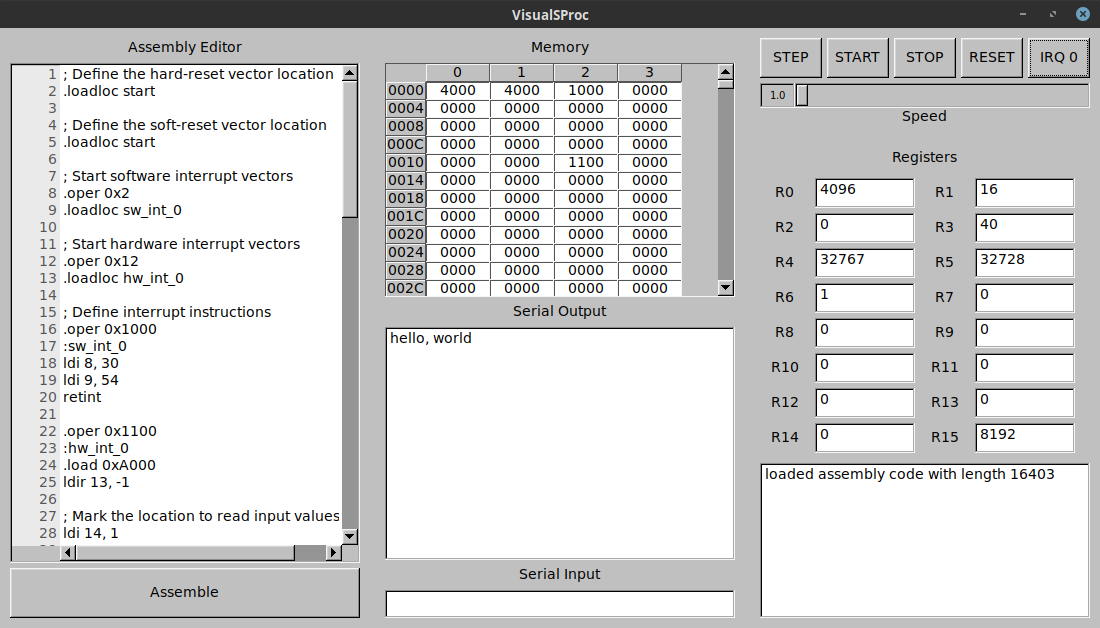
\includegraphics[width=5in]{images/visual-sproc.png}
	\caption{Main window of VisualSProc provides common tools for program writing}
	\label{fig:visual-sproc-main-page}
\end{figure}


\end{document}
